\documentclass[10pt,twocolumn,a4paper]{article}
\usepackage{graphicx}
\usepackage{tikz}
\usepackage{tikzscale}
\usepackage{parskip}
\usepackage{fullpage}
\usepackage{hyperref}
\usepackage{listings}
\usepackage{xcolor}
\usepackage{amsmath}
\usetikzlibrary{positioning}


\begin{document}

\title{Understanding through reversing}
\author{Denis Festa}
\date{\today}

\maketitle

\tableofcontents

\section{Introduction}
%
%%
%\begin{figure}[ht]
%	\centering
%	\includegraphics[scale=0.8]{memmap}
%	\caption{An example}
%	\label{fig:exmemmap}
%\end{figure}
%
%Before rebasing
%
%\begin{figure*}[ht]
%	\centering
%	\includegraphics[scale=0.8]{cor}
%	\caption{A grid with addresses}
%	\label{fig:cor}
%\end{figure*}
%
%This is a work on the reverse engineering of an esp32c6.

%

\section{Overview of the ESP32-C6}
\label{sec:overview}
From the technical reference:

ESP32-C6 is an ultra-low power and highly-integrated system that integrates:
\begin{itemize}
\item a high-performance 32-bit RISC-V single-core processor (HP CPU), four-stage pipeline, clock frequency
up to 160 MHz
\item a low-power 32-bit RISC-V single-core processor (LP CPU), two-stage pipeline, clock frequency up to
20 MHz
\end{itemize}
All internal memory, external memory, and peripherals are located on the HP CPU and LP CPU buses.

Features:
\begin{itemize}
\item Address Space
	\begin{itemize}
	\item 832 KB of internal memory address space accessed from the instruction bus or data bus
	\item 832 KB of peripheral address space
	\item 16 MB of external memory virtual address space accessed from the instruction bus or the data bus
	\item 512 KB of internal DMA address space
	\end{itemize}
\item Internal Memory
	\begin{itemize}
	\item 320 KB internal ROM
	\item 512 KB HP SRAM
	\item 16 KB LP SRAM
	\end{itemize}
\item External Memory
	\begin{itemize}
	\item Supports up to 16 MB external flash
	\end{itemize}
\item Peripheral Space
	\begin{itemize}
	\item 51 modules/peripherals in total
	\end{itemize}
\item GDMA
	\begin{itemize}
	\item 8 GDMA-supported modules/peripherals
	\end{itemize}
\end{itemize}

Here is a simplified diagram of the ESP32-C6's memory map.

\tikzset{every node/.append style={align=left, font=\LARGE}}
\tikzset{reserved/.style={fill=gray!30}}

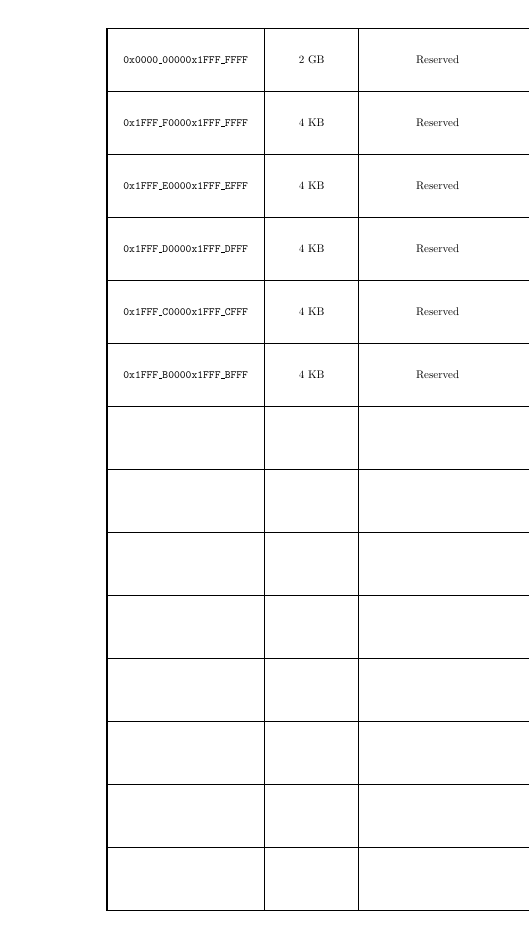
\begin{tikzpicture}[scale=0.4, every node/.append style={transform shape}]
\hspace*{1cm}
\draw (0,0) rectangle (15,-28);
% First column, address range
\draw (5,0) -- (5,-28);
% Second column, size 
\draw (8,0) -- (8,-28);
% Third column, title, from 8 to 15

% draw a row every 2 units from (0,i) to (15,i)
\foreach \i in {0,-2,...,-28}
	\draw (0,\i) -- (15,\i);

\node at (2.5,-1) {\texttt{0x0000\_0000}\\\texttt{0x1FFF\_FFFF}};
\node at (6.5,-1) {2 GB};
\node at (10.5,-1) {Reserved};

\node at (2.5,-3) {\texttt{0x1FFF\_F000}\\\texttt{0x1FFF\_FFFF}};
\node at (6.5,-3) {4 KB};
\node at (10.5,-3) {Reserved};

\node at (2.5,-5) {\texttt{0x1FFF\_E000}\\\texttt{0x1FFF\_EFFF}};
\node at (6.5,-5) {4 KB};
\node at (10.5,-5) {Reserved};

\node at (2.5,-7) {\texttt{0x1FFF\_D000}\\\texttt{0x1FFF\_DFFF}};
\node at (6.5,-7) {4 KB};
\node at (10.5,-7) {Reserved};

\node at (2.5,-9) {\texttt{0x1FFF\_C000}\\\texttt{0x1FFF\_CFFF}};
\node at (6.5,-9) {4 KB};
\node at (10.5,-9) {Reserved};

\node at (2.5,-11) {\texttt{0x1FFF\_B000}\\\texttt{0x1FFF\_BFFF}};
\node at (6.5,-11) {4 KB};
\node at (10.5,-11) {Reserved};

\end{tikzpicture}

And here follows another ...


\section{Hooking}
\label{sec:hooking}
Here we talk about hooking.


\newsavebox\funlmactxframe

\lstset{
	basicstyle=\ttfamily,
	columns=fullflexible,
	%frame=single,
	breaklines=true,
	postbreak=\mbox{\textcolor{red}{$\hookrightarrow$}\space},
}

\begin{lrbox}{\funlmactxframe}
\begin{lstlisting}
void lmacTxFrame(int param_1,int param_2)
{
    /*Decompiled code from the original libraries*/
    4000a06a 93 97 49 03 li     a5,0x34
    4000a06e b3 87 f5 02 mul    a5,a1,a5
    4000a072 01 11       c.addi sp,-0x20
    4000a074 22 cc       c.swsp s0,0x18(sp)
    4000a076 37 04 88 40 lui    s0,0x40880
    4000a07a 52 c4       c.swsp s4,0x8(sp)
    ...
}
\end{lstlisting}
\end{lrbox}

\newsavebox\funpatchlmactxframe
\begin{lrbox}{\funpatchlmactxframe}
\begin{lstlisting}
void patched_lmacTxFrame(int param_1,int param_2)
{
    /*Our patched version of lmacTxFrame*/
}
\end{lstlisting}
\end{lrbox}

\newsavebox\funactivation
\begin{lrbox}{\funactivation}
\begin{lstlisting}
void activation()
{
    /*Our activation function*/
    // lui+jalr to call_lmacTxFrame
    uint32_t lui_instr  = 0x4200c0b7;   // LUI instruction
    uint32_t jalr_instr = 0x1b4080e7;  // JALR instruction

    uint32_t *base_ppProcessTxQ = (uint32_t *) 0x4080e3fc;
    uint32_t offset_ppProcessTxQ = 0x70; // 0x4080e46c - 0x4080e3fc

    // ppProcessTxQ
    uint32_t *ppProcessTxQ_lui = \
        (uint32_t *)((char *)base_ppProcessTxQ +\
                     offset_ppProcessTxQ);
    uint32_t *ppProcessTxQ_jalr = \
        (uint32_t *)((char *)base_ppProcessTxQ +\
                     offset_ppProcessTxQ + 0x4);
    *ppProcessTxQ_lui = lui_instr;
    *ppProcessTxQ_jalr = jalr_instr;    
}
\end{lstlisting}
\end{lrbox}

\newsavebox\funcalllmactxframe
\begin{lrbox}{\funcalllmactxframe}
\begin{lstlisting}
/*Suppose the compiled code starts at 
  0x4200c1b4*/
void call_lmacTxFrame(int param_1,int param_2)
{
    /*Our function to call lmacTxFrame*/
    counter++; // A global counter of how 
               // many times lmacTxFrame is called
    /*Do some processing such as changing the
      channel before calling lmacTxFrame*/
    return lmacTxFrame(param_1,param_2);
    /* Or return patched_lmacTxFrame(param_1,param_2)
       in case we want to patch the original function*/
}
\end{lstlisting}
\end{lrbox}

\newsavebox\funprocesstxq
\begin{lrbox}{\funprocesstxq}
\begin{lstlisting}
void processTxQ()
{
    /*One among different functions from the 
      original library that calls lmacTxFrame*/
    4080e3fc 41 11       c.addi  sp,-0x10
    4080e3fe 26 c2       c.swsp  s1,0x4(sp)
    4080e400 06 c6       c.swsp  ra,0xc(sp)
    4080e402 22 c4       c.swsp  s0,0x8(sp)
    4080e404 aa 84       c.mv    s1,a0
    ... 
    4080e46c b7 a0 00 40 lui     ra,0x4000a
    4080e470 e7 80 a0 06 jalr    ra,ra,offset=0x06a lmacTxFrame 
    ...
}
\end{lstlisting}
\end{lrbox}


\newsavebox\funprocesstxqaft
\begin{lrbox}{\funprocesstxqaft}
\begin{lstlisting}
void processTxQ()
{
    /*One among different functions from the 
      original library that calls lmacTxFrame*/
    4080e3fc 41 11       c.addi  sp,-0x10
    4080e3fe 26 c2       c.swsp  s1,0x4(sp)
    4080e400 06 c6       c.swsp  ra,0xc(sp)
    4080e402 22 c4       c.swsp  s0,0x8(sp)
    4080e404 aa 84       c.mv    s1,a0
    ... 
    4080e46c b7 c0 00 42 lui     ra,0x4200c
    4080e470 e7 80 40 1b jalr    ra,ra,offset=0x1b4 call_lmacTxFrame 
    ...
}
\end{lstlisting}
\end{lrbox}

\newsavebox\funpropcode
\begin{lrbox}{\funpropcode}
\begin{lstlisting}
{
/* Proprietary code that calls 
   different functions among which
   those that call lmacTxFrame,
   such as ppProcessTxQ */
     ...
     ppProcessTxQ();
     ...
}
\end{lstlisting}
\end{lrbox}


\newsavebox\funmain
\begin{lrbox}{\funmain}
\begin{lstlisting}
void main()
{
    ...
    /* Before activation, the call flow
       is ppProcessTxQ -> lmacTxFrame */
    activation();
    /* After activation, the call flow
       is ppProcessTxQ -> call_lmacTxFrame
          -> lmacTxFrame (or patched_lmacTxFrame) */
    ...
}
\end{lstlisting}
\end{lrbox}


Here we show the use of an activation function to 
modify the flow of execution of a program by modifying 
directly original assembly code.

\begin{figure*}[ht]
\begin{tikzpicture}[scale=0.55, 
		    every node/.append style={transform shape}]
	\node[draw] (nfunmain) {\usebox\funmain};
	\node[draw, below=5cm of nfunmain] (nfunactivation) {\usebox\funactivation};
	\node[draw, right=6cm of nfunmain] (nfunprocesstxq) {\usebox\funprocesstxq};
	\node[draw, above=of nfunprocesstxq] (nfunpropcode) {\usebox\funpropcode};
	\node[draw, below=of nfunprocesstxq] (nfunlmactxframe) {\usebox\funlmactxframe};
	\node[draw, below=of nfunlmactxframe] (nfunprocesstxqaft) {\usebox\funprocesstxqaft};
	\node[draw, below=of nfunprocesstxqaft] (nfuncalllmactxframe) {\usebox\funcalllmactxframe};
	%\node[draw, below left=of nfuncalllmactxframe] (nfunlmactxframe) {\usebox\funlmactxframe};
	\node[draw, below=of nfuncalllmactxframe] (nfunpatchlmactxframe) {\usebox\funpatchlmactxframe};

	% using to for the edge between the nodes with in and out angles and text auto sloped
	\draw[->] (nfunmain) to[out=-100,in=100] node[auto,sloped] {} (nfunactivation);
	\draw[->, color=red] (nfunactivation) to[out=90,in=200] node[auto,sloped] {Injecting assembly} (nfunprocesstxq);
	\draw[->, color=red] (nfunprocesstxq) to[out=20, in=20, looseness=0.8] node[auto,sloped] {} (nfunprocesstxqaft);

	% Before activation
	\draw[->] (nfunpropcode) to[out=0, in=10] node[auto,sloped] {before \texttt{activation()}} (nfunprocesstxq);
	\draw[->] (nfunprocesstxq) to[out=0, in=10] node[auto,sloped] {} (nfunlmactxframe);
	\draw[->, color=blue] (nfunpropcode) to[out=10, in=10,looseness=0.8] node[auto,sloped,pos=0.2] {After \texttt{activation()}} (nfunprocesstxqaft);
	\draw[->, color=blue] (nfunprocesstxqaft) to[out=0, in=10] node[auto,sloped,] {} (nfuncalllmactxframe);
	\draw[->, color=blue] (nfuncalllmactxframe) to[out=180, in=180,looseness=0.5] node[auto,sloped] {} (nfunlmactxframe);
	

\end{tikzpicture}

\caption{Original function processTxQ and the function after activation}
\label{fig:workflowchange}

\end{figure*}



\section{Descriptors}

The libraries developed by Espressif create a linked structure of descriptors that
is used to point to the content of the bytes being sent or received.
Every packet is described by a triplet: a description of the packet, a pointer to the start of the packet
and a pointer to the next descriptor. Each element of the triplet is a 32-bit word, unfortunately
at the moment of writing it is not completely clear how the values in the description field are used
but it is enough for us to be able to send a custom frame with a length of our choice.
\newsavebox{\descriptor}
\begin{lrbox}{\descriptor}
\begin{lstlisting}
typedef struct __attribute__((packed)) descriptor {
	uint16_t _unknown_2 : 14;
	uint16_t length : 12;
	uint8_t _unknown_1 : 4;
	uint8_t has_data : 1;
	uint8_t owner : 1;
	void* frame;
	struct descriptor* next;
} descriptor;
\end{lstlisting}
\end{lrbox}
\usebox{\descriptor}
The first word of the descriptor, that is the description, is a 32-bit field 
that contains a bit indicating whether the packet is directed to the device,
it is relevant during the reception of frames and, unless we
are requiring a \textit{promiscuous mode}, when set to 0 the frame is discarded.
The second bit is used to indicate whether the bytes in the area actually contain 
meaningful data or if the content is garbage. The meaning of the following 4 bits, at the moment
of writing, is not clear. 
The length field is a 12-bit field that indicates the length of the frame and the last 14 bits,
at the moment of writing, are not clear.
The length represented in the 12 bits is comprehensive of the radiotap header, 
the 802.11 radio information, the frame content and the FCS.
In actuality, the lenght field in the description must be set to the length of the final desired
length minus 7, that is, when the description field is \texttt{0xfff} (4095) the length of the frame
will be 4102 bytes. The reason for this discrepancy of 7 bytes is not clear at the moment of writing.
It is important to notice how this is only one of the different places where the length of the frame
will be indicated, another place is in the first 4 bytes of the area referenced by the pointer to the packet:
that area starts with 2 words and the last 12 bits of the first word (little-endian speaking)
represent the length of the payload of the frame, that is, the length of the whole frame minus 15 bytes. 
Interestingly enough the radiotap header is not always 15 bytes long, but even when a 18 bytes 
long radiotap header is observed, the length of the payload is still 15 bytes less than the length of the frame.
A 18 bytes long radiotap header is observed when the data rate is set to some other values such as 6.5Mb/s, 13Mb/s, 65Mb/s...
and modulation techniques such as OFDM are used instead of DSSS as in the case of data rates such as 1 or 2 Mbps. 
% VERIFY THIS
% VERIFY THIS
The third place where the length of the frame is indicated is in the area of memory reserved to
peripheral registers. 
In case of certain data rates 
such as 1Mb/s, 2Mb/s, 6Mb/s, 12Mb/s, 48Mb/s, 54Mb/s...the address \texttt{0x600a5488} contains, in its last 12 bits (little-endian speaking),
the length of the payload of the frame (the length of the frame minus 15 bytes, the same value observed
at the beginning of the packet area).
In case of other data rates such as 6.5Mb/s, 13Mb/s, 65Mb/s... the address 
\texttt{0x600a5494} contains in its bits from the 20th to the 9th (12 bits) the same length as before.

\newsavebox{\memdescriptor}
\begin{lrbox}{\memdescriptor}
\begin{lstlisting}
0x4082d434: 0xc04a4000 0x4082d4a8 0x00000000 0x00000000
...
0x4082d4a8: 0x00000121 0x00000000 0xa74600d0 0xffffffff
0x4082d4b8: 0x4c40ffff 0xd85751ca 0xffffffff 0x0000ffff
...
// for some data rates
0x600a5488: 0x00000121 ...
// for other data rates
0x600a5494: 0x00012100 ...
...
\end{lstlisting}
\end{lrbox}
\usebox{\memdescriptor}
We underline that the values written above are only partially \textit{true},
in particular the values in the two peripheral registers only contain the length value
and not the remaining important informations regarding the data rate itself and 
other yet to be discovered informations.  
The example above shows a descriptor whose description field contains a length value
of 0x129 (297 bytes), in fact the value 
\texttt{110000 000100101001 00000000000000} of the description field contains
as the length value the 12 bits \texttt{000100101001} that in decimal is 297,
this reflects to a real length of $297+7=304$ bytes and to a payload length of $304-15=289$ bytes
that is written as \texttt{0x121} at the beginning of the area referenced by the pointer to the frame and 
in the peripheral register (either \texttt{0x600a5488} or \texttt{0x600a5494}).
In the example above the descriptor does not point to a next descriptor, meaning it is the last
of a queue.


\section{Binary patching}

While reversing the original implementation of wifi functionalities, it was useful to reimplement 
some core functions ourselves to better understand them, moreover, if the goal is to create
an open source driver for the wifi whip, reimplementing binary code in a more readable form
(like C) is the main step.
The open source software Ghidra (developed by the NSA) was used to obtain 
a disassembled version of the binary code. Although powerful, Ghidra is not perfect and
sometimes the disassembled code is not perfect, e.g., it might not recognize the exact
number of parameters of a function. 
We will show an example of one of the most important function we reimplemented,
\texttt{lmacTxFrame}, responsible for sending a frame, also mentioned in the section \ref{sec:hooking}.
The code below is a simplified version of the disassembly obtained from Ghidra,
some function calls were not trivial to understand because
the symbolic names were not available, so we had to mimic the calls
using function pointers to addresses available in the binary and 

\lstset{
	basicstyle=\ttfamily,
	columns=fullflexible,
	breaklines=true,
	postbreak=\mbox{\textcolor{red}{$\hookrightarrow$}\space},
}

%\newsavebox{\funlmactxframe}
%\begin{lrbox}{\funlmactxframe}
\begin{lstlisting}

void lmacTxFrame(int param_1,int param_2)

{
  undefined uVar1;
  ushort uVar2;
  int iVar3;
  uint uVar4;
  uint *puVar5;
  int iVar6;
  int iVar7;
  uint uVar8;
  int *piVar9;
  
  gp = coex_schm_ble_mesh_standby_\
          bt_a2dp_paused_wifi_connecting;
  piVar9 = (int *)(param_2 * 0x34 + 0x4087f840);
  if (*(char *)(param_2 * 0x34 + 0x4087f852) != '\x04') {
    ...
    iVar3 = (**(code **)(_pp_wdev_funcs + 0xe4))(param_1,*(code **)(_pp_wdev_funcs + 0xe4));
    puVar5 = *(uint **)(param_1 + 0x34);
    ...
    if ((((int)(*puVar5 << 0x13) < 0) && (*(char *)(param_2 * 0x34 + 0x4087f852) == '\x03')) &&
       (*(byte *)(_lmacConfMib_ptr + 0x2a) <= *(byte *)((int)puVar5 + 5))) {
      *puVar5 = *puVar5 & 0xffffefff | 0x100;
      ...
    }
    ...
    (**(code **)(_pp_wdev_funcs + 0xe8))(piVar9,0,*(code **)(_pp_wdev_funcs + 0xe8));
  }
  ...
}
\end{lstlisting}
%\end{lrbox}

%\usebox{\funlmactxframe}

The code above is the corrispondent reimplementation in C, again simplified in
order to mirror only the displayed portions of the disassembly.
%\newsavebox{\funpatchlmactxframe}
%\begin{lrbox}{\funpatchlmactxframe}
\begin{lstlisting}

void patched_lmacTxFrame(int param_1, int param_2)
{
  uint8_t uVar1;
  uint16_t uVar2;
  int iVar3;
  uint32_t uVar4; 
  uint32_t *puVar5;
  int iVar6;
  int iVar7;
  uint32_t uVar8;
  int *piVar9;

  ESP_LOGI(TAG, "patched_lmacTxFrame: address: 0x%"PRIx32"", (uint32_t)param_1);

  piVar9 = (int *)(param_2 * 0x34 + (char *)our_instances_ptr); // Calculating the instance structure
  if (*(char *)(param_2 * 0x34 + (char *)our_instances_ptr + 0x12) != '\x04') {
    ...
    // Call an external function at address 0xXXXXXXXX, e.g., _pp_wdev_funcs + 0xe4
    iVar3 = patched_lmacIsLongFrame(param_1); // Replace with actual address
    puVar5 = *(uint32_t **)(param_1 + 0x34);
    ...
    // Check another condition and modify the frame if needed
    if ((((int)(*puVar5 << 0x13) < 0) && (*(char *)(param_2 * 0x34 + (char *)our_instances_ptr + 0x12) == '\x03')) && (*(uint8_t *)(lmacConfMib_ptr + 0x2a) <= *(uint8_t *)((int)puVar5 + 5))) {
      *puVar5 = (*puVar5 & 0xffffefff) | 0x100;
      ...
    }
    ...
    patched_lmacSetTxFrame(piVar9, 0); // Replace with actual address
  }
 ...
}
\end{lstlisting}
%\end{lrbox}

%\usebox{\funpatchlmactxframe}

A first example of discrepancy between the closed source disassembly and the
open source reimplementation is the use of the symbol \texttt{our\_instances\_prt}
that in the original code is obfuscated by the address \texttt{0x4087f840};
this might happen because the specific function \texttt{lmacTxFrame} is
located in the rom of the chip and the address is fixed, whereas 
in another function located in ram (\texttt{lmacTxDone}, which we will mention later) the symbol
\texttt{our\_instances\_ptr} is used.
We could have used the address \texttt{0x4087f840} directly, but we decided to use the symbol because,
although not in this case, values of the addresses might change depending even on the specific
build of the program, and using the symbol, in addition to being resilient to addresses changes,
makes the code more readable.
Another difference is the way some functions are called,
e.g. \texttt{(**(code **)(\_pp\_wdev\_funcs + 0xe8))(piVar9,0,*(code **)(\_pp\_wdev\_funcs + 0xe8));}
is a call to a function pointer whose address is stored at \texttt{\_pp\_wdev\_funcs + 0xe8},
here it is possible to get confused by Ghidra's notation. 
Ghidra suggests the value \texttt{0x4087ff70} when hovering on
the symbol \texttt{\_pp\_wdev\_funcs}, but it is not
always easy to distinguish whether \texttt{0x4087ff70} is actually
the address at which the symbol is stored or the constant
value of the symbol itself, therefore the sum \texttt{\_pp\_wdev\_funcs + 0xe8}
might be interpreted in two different ways:
\begin{itemize}
\item getting the address of \texttt{\_pp\_wdev\_funcs},
which Ghidra automatically suggests to be \texttt{0x4087ff70}, then adding
\texttt{0xe8} to it, resulting in \texttt{0x40880058}, and using this result as
the address of the function pointer;
\item getting the address of \texttt{\_pp\_wdev\_funcs}, loading the value at that address
(\texttt{*(uint32\_t *)0x4087ff70} or \texttt{*(uint32\_t *)\&\_pp\_wdev\_funcs}),
adding \texttt{0xe8} to the value loaded from \texttt{0x4087ff70}, and using this result as
the address of the function pointer.
\end{itemize}
The only way to know which interpretation is correct is to look at the assembly code,
we will paste just the needed portion below:

%\newsavebox{\funlmactxframeassembly}
%\begin{lrbox}{\funlmactxframeassembly}
\begin{lstlisting}
4000a098 b7 04 88 40     lui        s1,0x40880
...
4000a0bc 83 a7 04 f7     lw         a5,-0x90(s1=>pp_wdev_funcs)
4000a0c0 56 85           c.mv       a0,s5
4000a0c2 83 a7 47 0e     lw         a5,0xe4(a5)
4000a0c6 82 97           c.jalr     a5
\end{lstlisting}
%\end{lrbox}

%\usebox{\funlmactxframeassembly}

Now it becomes clear that the correct interpretation is the second one,
we first need to load the value at the address suggested by Ghidra \texttt{0x4087ff70},
which is not the value of the symbol itself but the address at which the symbol is located,
in assembly the first portion of the address is loaded into the register \texttt{s1} as
the value \texttt{0x40880000}, then the exact address is represented by
the \texttt{-0x90} offset from \texttt{s1}, which leads to \texttt{0x4087ff70},
the instruction \texttt{lw a5,-0x90(s1)} loads the value at \texttt{0x40880000-0x90} into \texttt{a5},
we know we have to load 4 bytes because to load a 16-bit value we would have read the instruction
\texttt{lhu a5,-0x90(s1)} and to load an 8-bit value we would have read the instruction
\texttt{lb a5,-0x90(s1)}. 
The value loaded is then used again as an address in \texttt{lw a5,0xe4(a5)} to load
the actual function pointer address into \texttt{a5}. 
The \texttt{jalr a5} performs the jump-and-link operation to call the function at the address
stored in \texttt{a5}.
After correctly reimplementing the function call, we could confirm that the function being
called was \texttt{lmacSetTxFrame} with GDB and we could substitute in the code an explicit
call using that symbol (or our patched version of it, \texttt{patched\_lmacSetTxFrame}).

A similar reasoning can be applied to the portion of code using the symbol \texttt{\_lmacConfMib\_ptr}.
First, it is important to understand the assembly and it might be preferable to use hardcoded addresses,
then with some \texttt{printf} debugging it is possible to tell whether the hardcoded address
is the value of the symbol being investigated or the address at which the symbol is stored.




\section{Wi-Fi in the esp32c6}
\label{sec:wifiinesp32c6}
Our main goal was to understand the way 802.11 frames are sent
and received by the esp32c6.
The libraries provided by Espressif rely on FreeRTOS,
a real-time operating system that offers the programmers a
set of functions to manage tasks, queues, semaphores and other 
resources.

The first step of our investigation was to
build a sample application that would allow us to send and
receive 802.11, fortunately Espressif provides a lot of
useful examples that we could use as a starting point,
we wrote a sample application that would connect to an
access point and download the page \url{http://example.com}.
By building the application we could obtain the ELF file
that we could analyze with Ghidra.
The ELF alone was not enough, some functions were not
available in the ELF (among which, \texttt{lmacTxFrame} which 
sends frames), so we had to dump the rom and import
it into Ghidra.
Although the great help of Ghidra, some functions were
not easily understandable because they would call other 
functions by means of unreferenced function pointers,
so we had to use GDB to understand the flow of the program.
Later, we decided to focus on sample programs that would
rely on the \textit{espnow} protocol, the reason was that
espnow is a protocol developed by Espressif that allows
two or more esp32 to communicate without the need of an
access point, this would supposedly simplify the analysis
because we would not have to deal with the complexity of
the full TCP/IP stack but only with the second layer of it,
the MAC layer, in particular, the 802.11 protocol.
We built a sample application that would send and receive 
espnow frames and verified that the frames were correctly
sent and received between two esp32c6.
With some sessions of debugging with GDB we could individuate
the function \texttt{lmacTxFrame} as the responsible for sending
frames (in actuality, many functions are involved in the process
but \texttt{lmacTxFrame} is the one that contains a
\texttt{store-word} instruction that writes a value to an
MMIO register that triggers the sending of the frame: \texttt{0x600a4d6c}).
We talk about how we intercepted this function in \ref{sec:hooking} to understand
when it is called.
Once the \textit{lowest level} function was found, we binary patched some functions
starting both from the \textit{top} level of abstraction and
the \textit{bottom} level of abstraction, hoping to find 
at a certain point a \textit{junction} where the two paths would meet.
Starting from the top level of abstraction, we patched:
\begin{itemize}
\item \texttt{esp\_now\_send}
\item \texttt{mt\_send}
\item \texttt{ieee80211\_send\_action\_vendor\_spec}
\item \texttt{ieee80211\_post\_hmac\_tx}
\item \texttt{pp\_post}
\end{itemize}
Starting from the bottom level of abstraction, we patched:
\begin{itemize}
\item \texttt{lmacTxFrame}
\item \texttt{lmacSetTxFrame}
\item \texttt{lmacIsLongFrame}
\end{itemize}
We could not find a junction between the two paths because,
although we understood that \texttt{lmacTxFrame} is called 
by \texttt{ppProcessTxQ} which is again called by \texttt{ppTask},
we could not find a way to call \texttt{ppTask}.
After some more debugging, we realized that \texttt{ppTask} is
exactly the main task handling the Wi-Fi features of the esp32c6
(and the esp32 in general).
The function \texttt{ppTask} runs in a thread which we will refer
to as \textit{wifi thread}, it basically keeps listening over
a shared queue for events and, based on the received event, it
calls the appropriate function.

Our objective became to substitute \texttt{ppTask} with a simpler implementation
that would allow us to send and receive 802.11 frames, at the moment of writing,
we have a demo that does not work resiliently, in order to investigate why 
we changed our demo to work on a single thread, without a dedicated
task that listens for events but by calling directly the functions needed 
to send and receive frames: we reached a point where we can have our demo
working for at least half an hour if we print logs to the console but 
then it stops working when we remove the logs, suggesting that a delay is
needed in order to keep the system working.
Once we will understand the reason for this, we might be able to revert
to the multi-threaded approach.
We will delve more into our demo later in \ref{sec:demo}.




\section{Our demo}
\label{sec:demo}

\end{document}

